\section{Results}

\subsection{Evidence is organized by estimand and evidence tier}

The manuscript evidence is separated into current-recording observations,
single-reviewer candidate calls, identity-aware interpretation, implementation
audits, and exact-truth simulation. Table~\ref{tab:venue-evidence-map} records
which results are main evidence and which remain provisional, computational, or
excluded. This prevents occurrence-level B58 sensitivity from being conflated
with site-level review yield, canonical-collapsed sensitivity, or an unrelated
global reranking budget.

\begin{table*}[!htbp]
\centering
\caption{Experimental inclusion and evidence-status matrix. P denotes a known
positive and U an unlabeled candidate, not a verified negative.}
\label{tab:venue-evidence-map}
\footnotesize
\renewcommand{\arraystretch}{0.96}
\begin{tabularx}{\textwidth}{>{\raggedright\arraybackslash}p{0.18\textwidth}
  >{\raggedright\arraybackslash}p{0.22\textwidth}
  >{\raggedright\arraybackslash}p{0.27\textwidth}
  >{\raggedright\arraybackslash}X}
\toprule
Evidence block & Unit and population & Estimand or protocol & Manuscript status \\
\midrule
Known-positive retrieval & \VenueCohortOccurrences{} occurrence geometries at
\VenueCohortSites{} sites & Any-lane match across three independently truncated
per-burst B\VenuePerLaneBudget{} lists & Main current-recording sensitivity;
not precision \\
Canonical grouping & \VenueCanonicalOccurrences{} occurrence rows & Prespecified
ROI-010/015 grouping sensitivity & Secondary sensitivity; primary geometry is
unchanged \\
Candidate review & \VenueReviewedCandidates{} detector-selected U sites & One
blinded reviewer; four normalized call classes & Provisional,
awaiting independent review and adjudication \\
Identity audit & \VenueStrictMissed{} all-lane misses & Six-pixel identity guard
and per-burst B\VenueCounterfactualBudget{} availability counterfactual &
Reviewed current-recording interpretation; small descriptive groups \\
Numerical audits & \VenueCohortSites{} centers over
\VenueAuditFrames{} frames & Long-delay inversion and local-standardization
reproduction & Numerical implementation support; not source separation \\
Exact-truth simulation & \VenueMovieBenchmarkCount{} factorial and
\VenueFamilyHoldoutCount{} mechanism-shift movies, plus a twelve-family suite &
One-to-one identity matching under known simulated truth & Computational
mechanism evidence; not biological transfer \\
Late engineering runs & Contextual, background-model, and Feature Atlas screens
& Same-recording feasibility or exploratory reranking & Excluded from main
claims unless registered, evidence-bound, and scientifically audited \\
\bottomrule
\end{tabularx}
\end{table*}

\subsection{The recording contains strong shared burst structure}

Across the \VenueCohortOccurrences{} confirmed occurrences, Raw traces contained
a strong event-aligned population waveform that was also expressed in nearby
tissue (Fig.~\ref{fig:venue-representations}). Local ROI-minus-annulus
subtraction retained event-associated amplitude, but the residual waveform was
not universal across sites. An exploratory shape-only taxonomy selected two
within-recording measurement phenotypes containing
\VenueTraceClassOneSites{} and \VenueTraceClassTwoSites{} sites. The registry
marks this claim provisional, the groups are not neuronal cell types, and their
leave-one-burst-out persistence was imperfect.

The registered long-delay temporal embedding was numerically invertible at the
audited sites, with maximum sitewise inversion root-mean-square error
$\VenueLongDelayInversionRMS$. Reproduction of the saved local-standardization
center traces agreed with the saved CUDA output at RMSE $\VenueLSRMSE$ and
maximum absolute error $\VenueLSMaxError$; the recorded scale floor was inactive
at all \VenueCohortSites{} audited centers over the \VenueAuditFrames-frame
interval. These checks validate numerical implementation and provenance, not
denoising or biological source separation. A distinct legacy two-frame operator
audit remains provisional and is reported only in the Appendix.

\subsection{Known-positive recovery is strong but does not identify precision}

At the frozen per-burst \(B=\VenuePerLaneBudget\) operating point, each of the
carrier, coherence, and lag-2 recurrence lists was evaluated independently. The
any-lane union recovered \VenueStrictRecovered{} of
\VenueCohortOccurrences{} confirmed occurrences, giving strict known-positive
sensitivity \VenueStrictSensitivity{} (Fig.~\ref{fig:venue-known-positive}).
The separately defined canonical-collapsed sensitivity was
\VenueCanonicalRecovered/\VenueCanonicalOccurrences{}
(\VenueCanonicalSensitivity). The first result is not a global top-58 list, and
neither denominator includes an exhaustive count of false positives.

The harder frame-level event-versus-guarded-quiet-reference assay ranked Raw
first, with site-weighted AUC \VenueRawAUC{} and a 95\% site-bootstrap interval
of \VenueRawAUCLow--\VenueRawAUCHigh. Carrier, coherence, and lag-2 recurrence
followed at \VenueCarrierAUC, \VenueCoherenceAUC, and \VenueLagAUC,
respectively. All six prespecified compact spatial-challenge features had
positive site-bootstrap intervals for true-center minus same-field
baseline-matched displaced AUC. These results support temporal retrieval and
localized measurement structure; quiet frames and displaced tissue were not
exhaustively shown to be biologically inactive.

\begin{figure*}[!htbp]
  \centering
  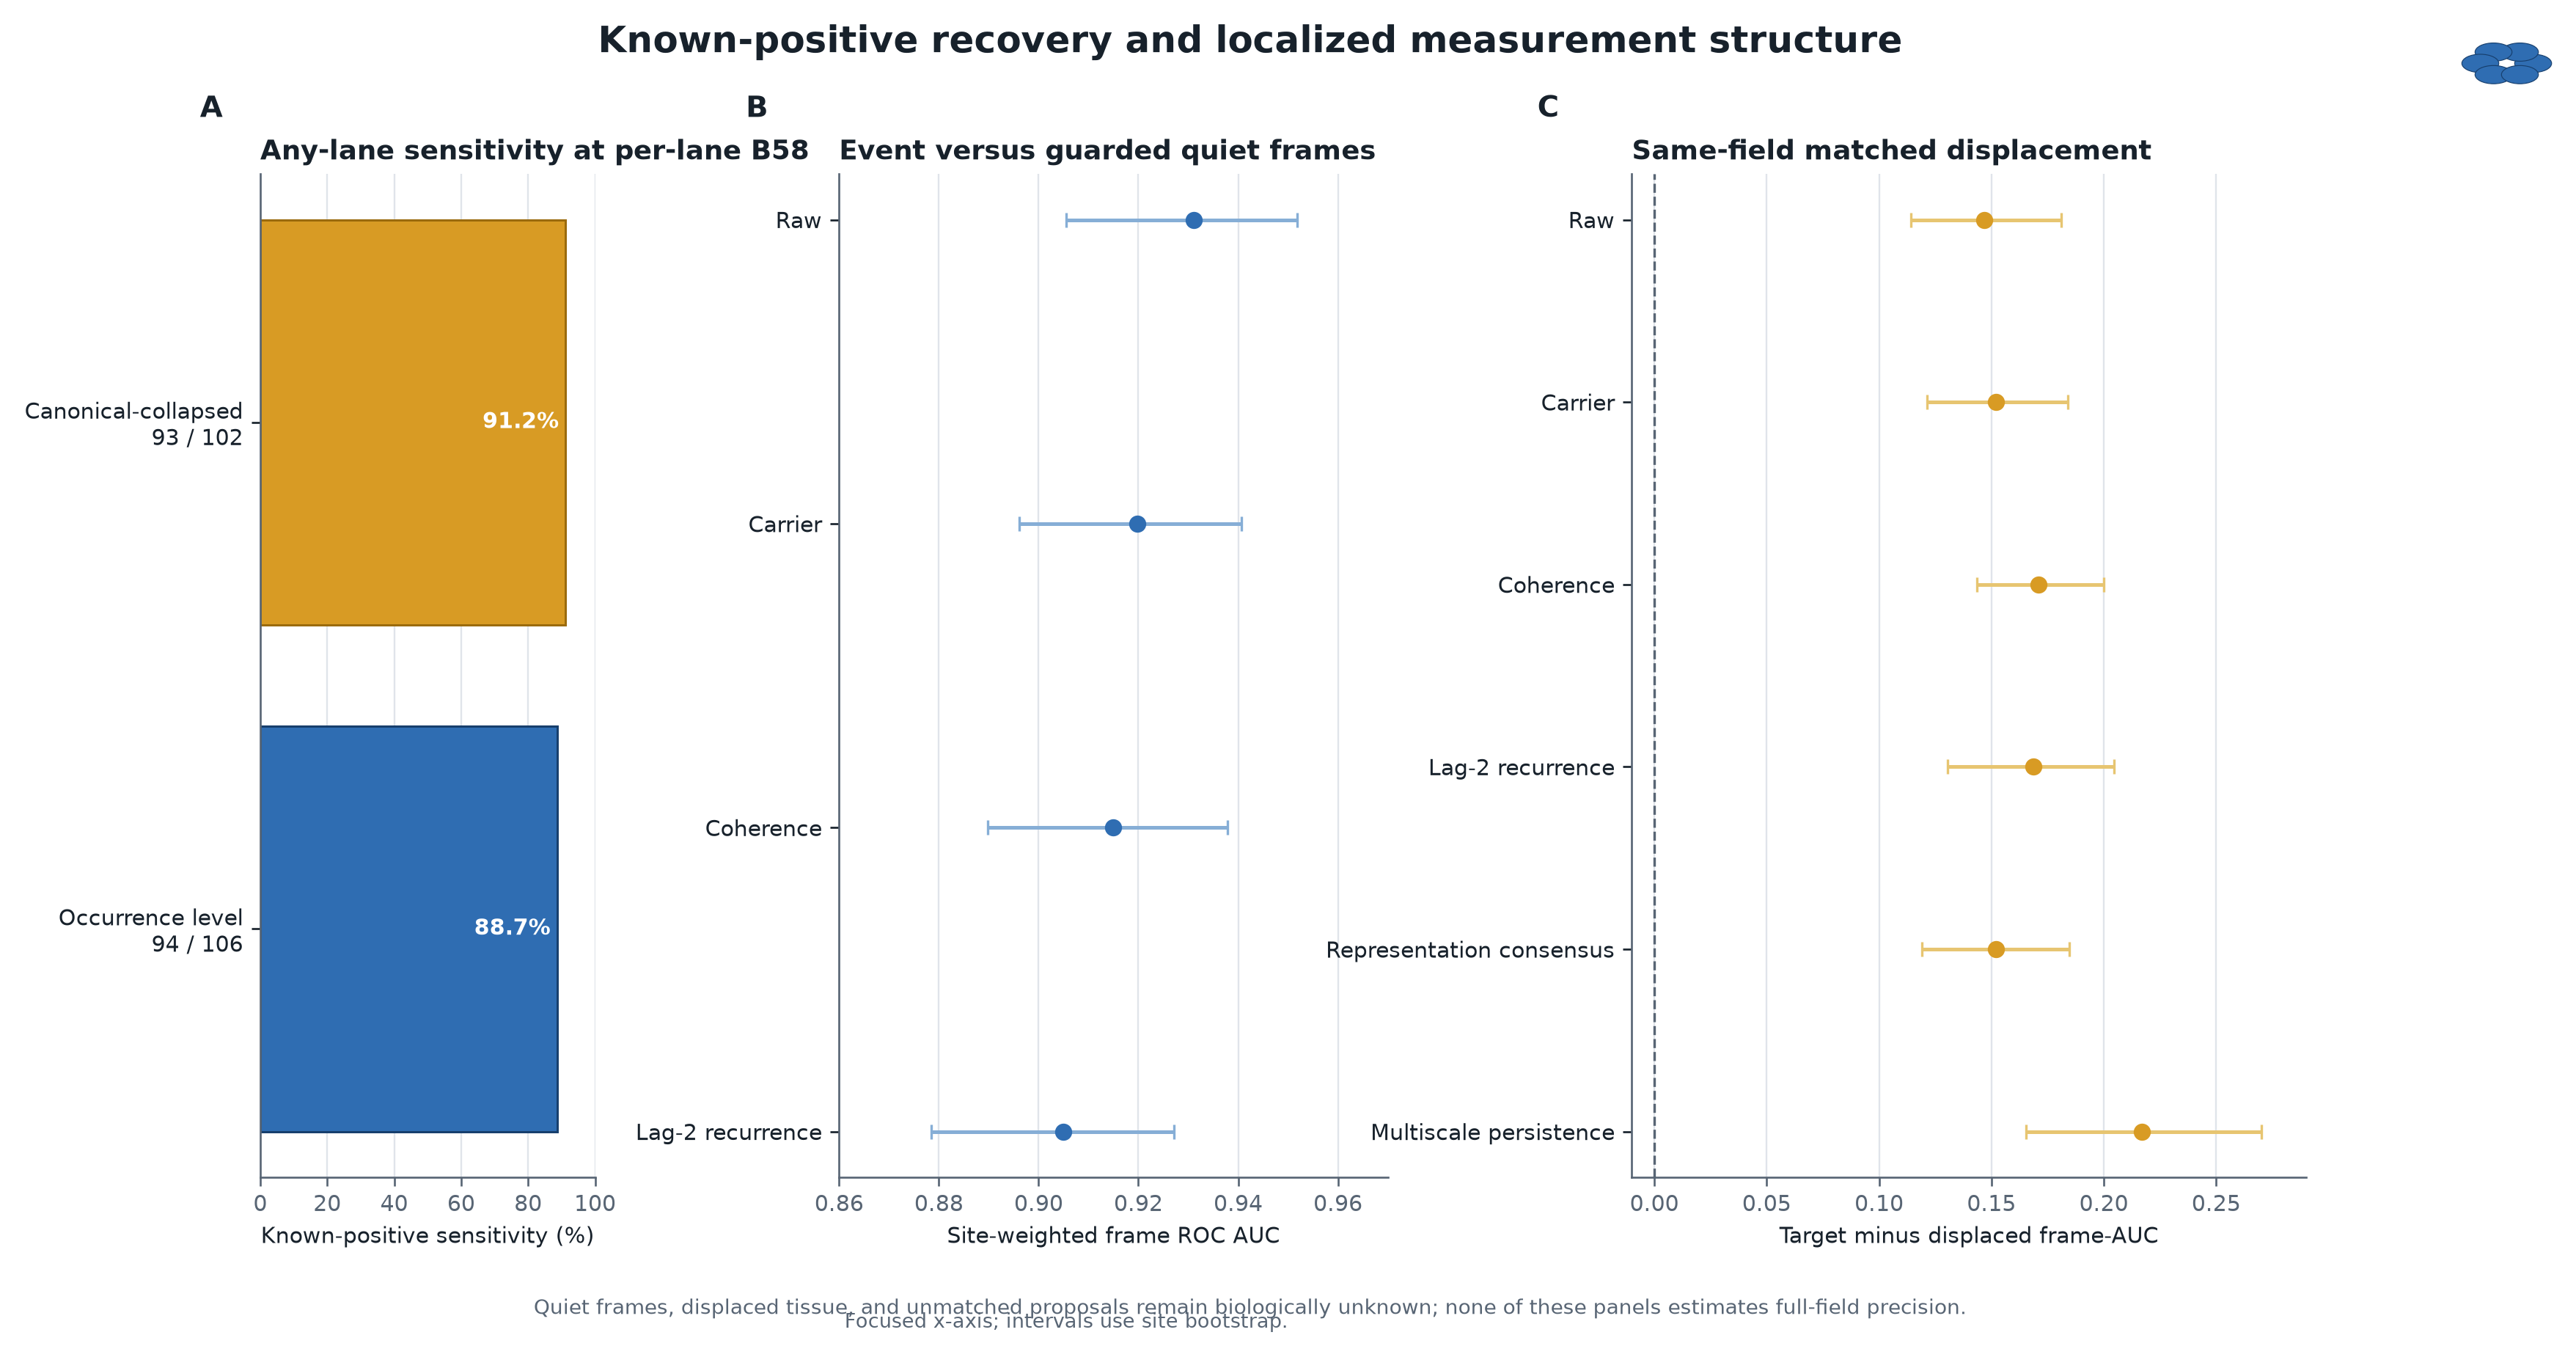
\includegraphics[width=\textwidth]{figures/venue/fig03_known_positive_evaluation.png}
  \caption{Known-positive recovery and localized measurement structure.
  Panel A explicitly reports an any-lane union across three independently
  evaluated per-burst B\VenuePerLaneBudget{} lists. Panel B reports
  event-versus-guarded-quiet-reference AUC with site-bootstrap intervals. Panel C
  reports target-minus-displaced frame-AUC. None of these panels estimates
  full-field precision or biological specificity.}
  \label{fig:venue-known-positive}
\end{figure*}

\subsection{Blinded review identifies provisional candidates with broader appearances}

The post-canonical-v7 review batch comprised \VenueReviewedCandidates{}
previously unmatched sites, none of which was a canonical-v7 positive target.
One blinded reviewer assigned \VenueReviewDefinite{} definite-neuron,
\VenueReviewProbable{} probable-neuron, \VenueReviewUncertain{} uncertain, and
\VenueReviewArtifact{} unlikely/artifact-or-noise calls
(Fig.~\ref{fig:venue-candidate-review}). Definite plus probable yielded
\VenueReviewLikely/\VenueReviewedCandidates{} provisional likely-neuron calls.
This is a detector-selected, single-reviewer yield, not detector precision, an
update to the \VenueCohortOccurrences-positive cohort, or
\VenueReviewLikely{} independently validated new identities. It is also distinct
from an earlier 18-item B005/B006 adjudication subset; the two batches are not
pooled.

The positive and probable calls included small and discrete appearances, a
low-signal-to-noise candidate, and a crescent or possibly multi-source footprint.
Artifact adjacency and stronger neighboring sources remained important sources
of uncertainty. The candidate-priority score was designed to elevate evidence,
ambiguity, and crowding rather than estimate neuron probability. Relative to the
single reviewer's provisional dichotomy, its descriptive AUC was
\VenueReviewPriorityAUC. Several definite calls received low priority, whereas
neighbor-confounded sites were promoted, demonstrating that review value and
biological probability are different targets.

\begin{figure*}[!htbp]
  \centering
  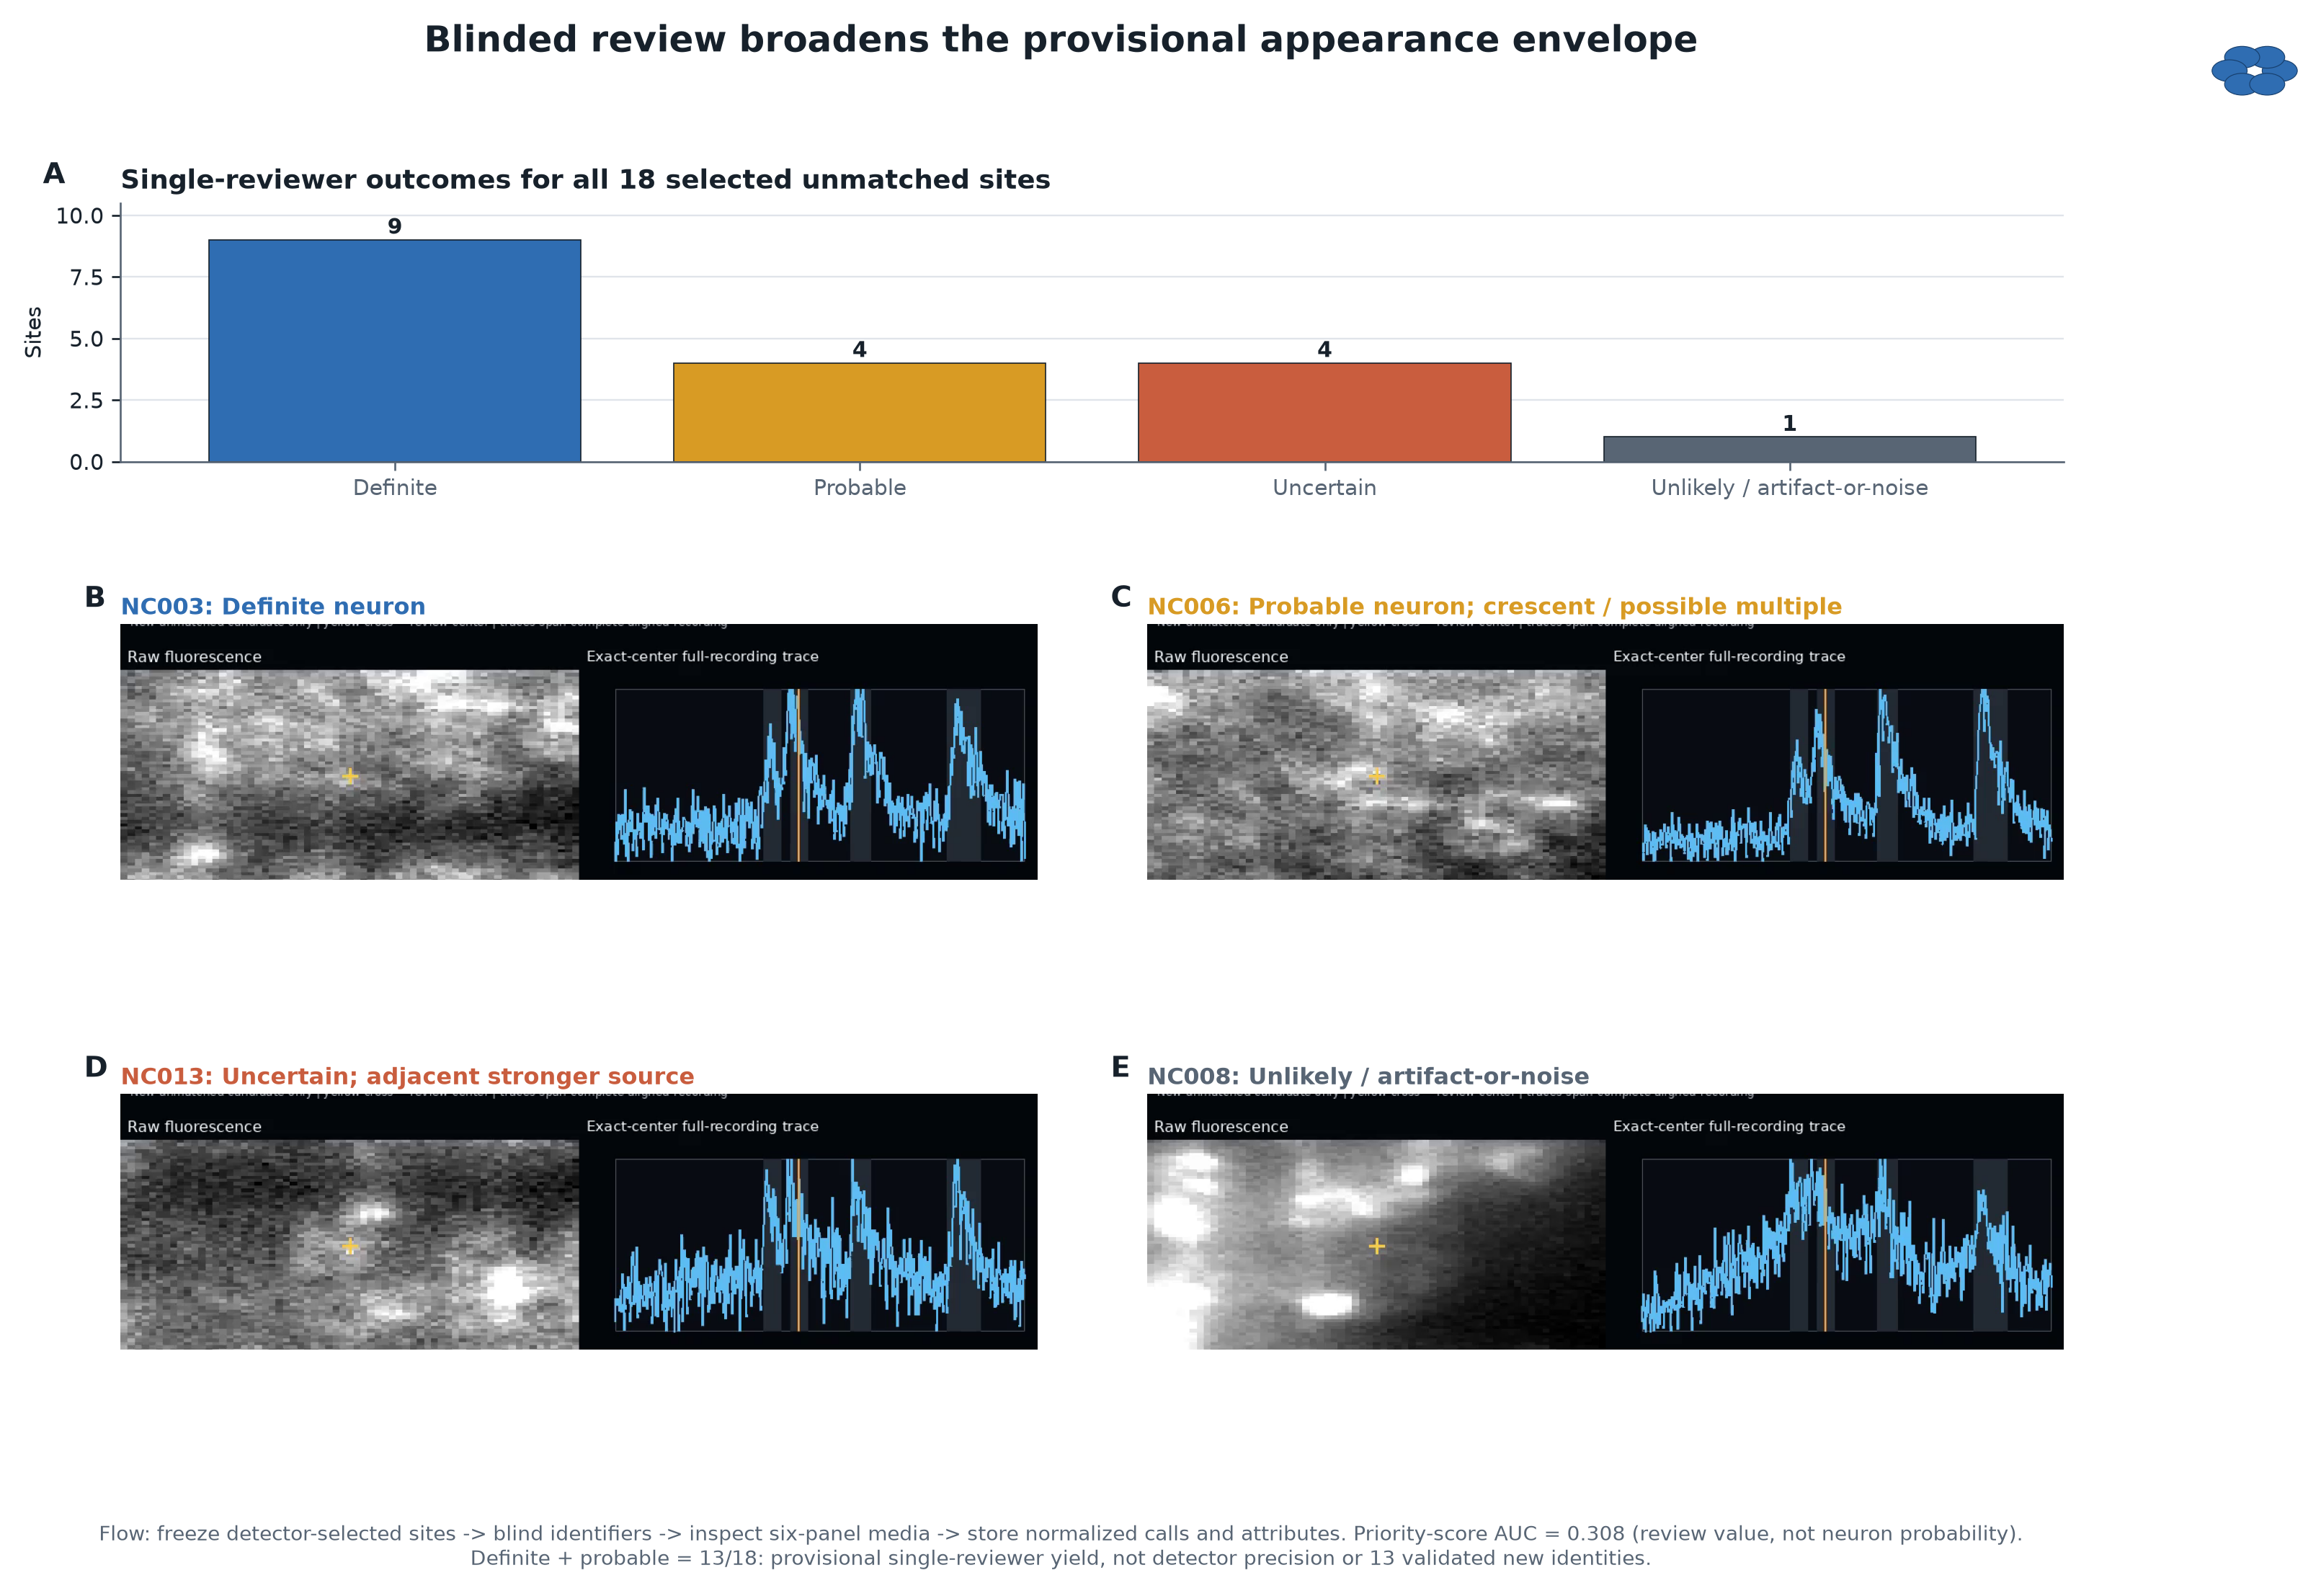
\includegraphics[width=\textwidth]{figures/venue/fig04_candidate_review.png}
  \caption{Selected unmatched-candidate review. The bar chart includes all
  \VenueReviewedCandidates{} single-reviewer outcomes; images show representative
  definite, probable, uncertain, and unlikely or artifact/noise calls. The
  observed \VenueReviewLikely/\VenueReviewedCandidates{} likely-neuron fraction
  is provisional selected-batch yield, not a precision estimate or a count of
  validated new biological identities.}
  \label{fig:venue-candidate-review}
\end{figure*}

\subsection{Identity guards overturn most apparent recentering gains}

Among the \VenueStrictMissed{} occurrences missed by all per-burst
B\VenuePerLaneBudget{} lanes, local consensus search produced
\VenueSameIdentityCollision{} candidates that collided with another geometry
from the same canonical identity and \VenueOtherIdentityCollision{} that
collided with a different labeled identity. Only \VenueIdentityClear{} were
identity-clear within the six-pixel guard. Thus,
\VenueIdentityCollision/\VenueStrictMissed{} apparent signal improvements could
not be interpreted as correction of the original neuron center: the optimized
measurement moved toward an already labeled source
(Fig.~\ref{fig:venue-identity-misses}).

The identity-clear cases remained hypotheses. ROI 19 was the cleanest
localization candidate; ROI 25 was directionally consistent but morphologically
irregular; ROI 22 was noise dominated; and ROI 27 lay in a crowded region
compatible with non-maximum suppression. No identity-clear miss had a frozen
candidate within eight pixels through per-burst
\(B=\VenueCounterfactualBudget\) in any audited lane. These cases are therefore
proposal-absence cases in the frozen outputs, not B58 reranking failures.

Median multi-neighbor variance explained was \VenueCollisionNeighborRtwo{} for
collision candidates and \VenueClearNeighborRtwo{} for identity-clear
candidates. Cross-stage displacement directions were also more consistent for
collisions (median cosine \VenueCollisionDirectionCosine) than identity-clear
cases (\VenueClearDirectionCosine). With group sizes
\VenueIdentityCollision{} and \VenueIdentityClear, none of three prespecified
exact descriptive permutation tests was small; these patterns remain
exploratory.

\begin{figure*}[!htbp]
  \centering
  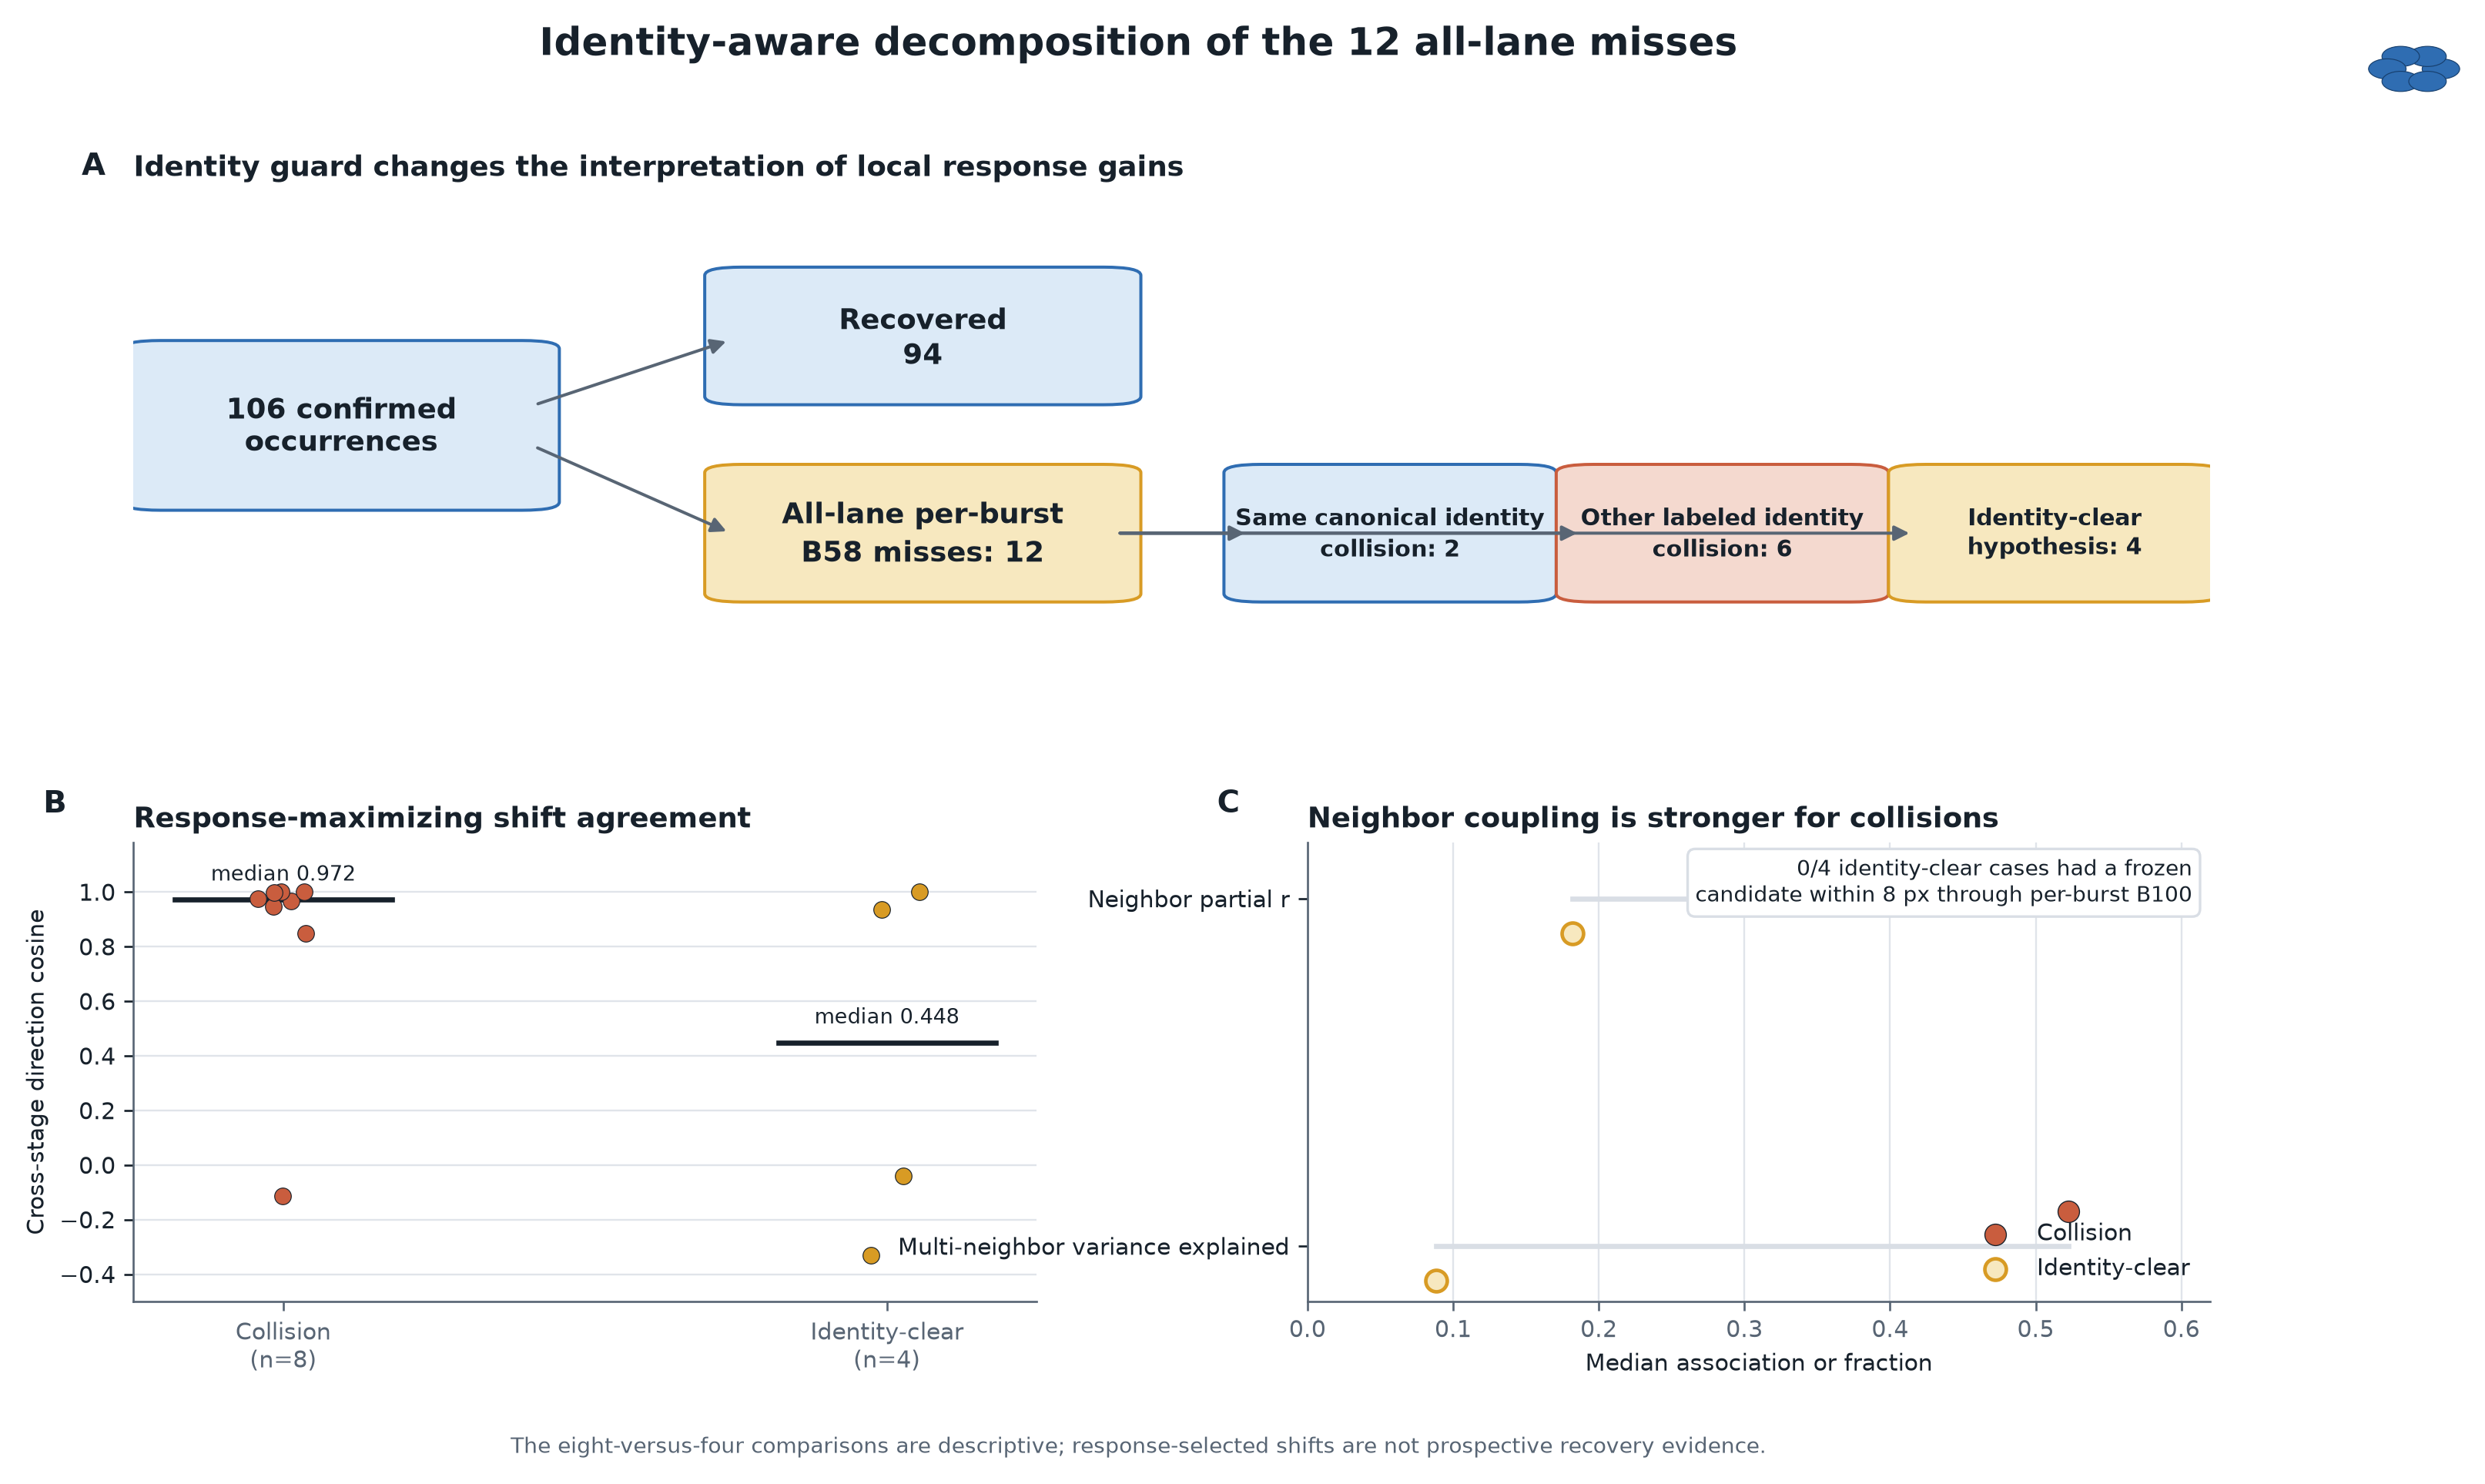
\includegraphics[width=\textwidth]{figures/venue/fig05_identity_aware_misses.png}
  \caption{Identity-aware failure decomposition. The
  \VenueStrictMissed{} all-lane misses divide into
  \VenueSameIdentityCollision{} same-canonical-identity collisions,
  \VenueOtherIdentityCollision{} other-labeled-identity collisions, and
  \VenueIdentityClear{} identity-clear hypotheses. Direction agreement,
  neighboring-trace association, and per-burst B\VenueCounterfactualBudget{}
  availability are descriptive diagnostics. Increased response after
  recentering is not recovery when a shift crosses identity.}
  \label{fig:venue-identity-misses}
\end{figure*}

\subsection{Exact-truth simulations resolve feature roles and expose limits}

In the \VenueMovieBenchmarkCount-movie factorial benchmark, the combined
carrier--spatial-context--kinetic stack had the highest identity-matched F1 at
budget 4 (\VenueMovieCombinedFone), whereas spatial context gave lower duplicate
counts and better localization. Under the separate
\VenueFamilyHoldoutCount-movie mechanism-shift benchmark, spatial context had
the highest F1 in every generator family and a mean F1 of
\VenueFamilySpatialFone{} versus \VenueFamilyCombinedFone{} for the equal-weight
combined stack (Fig.~\ref{fig:venue-exact-truth}). The twelve-family challenge
suite further identified crescent morphology (spatial-context pixel AUC
\VenueCrescentAUC), close unequal-amplitude sources, source-count-free stopping,
parameter stability, spectral noise realism, and kinetic directionality as
specific limits. These registered results are exact-truth computational evidence
and are not presented as biological external validation.

\begin{figure*}[!htbp]
  \centering
  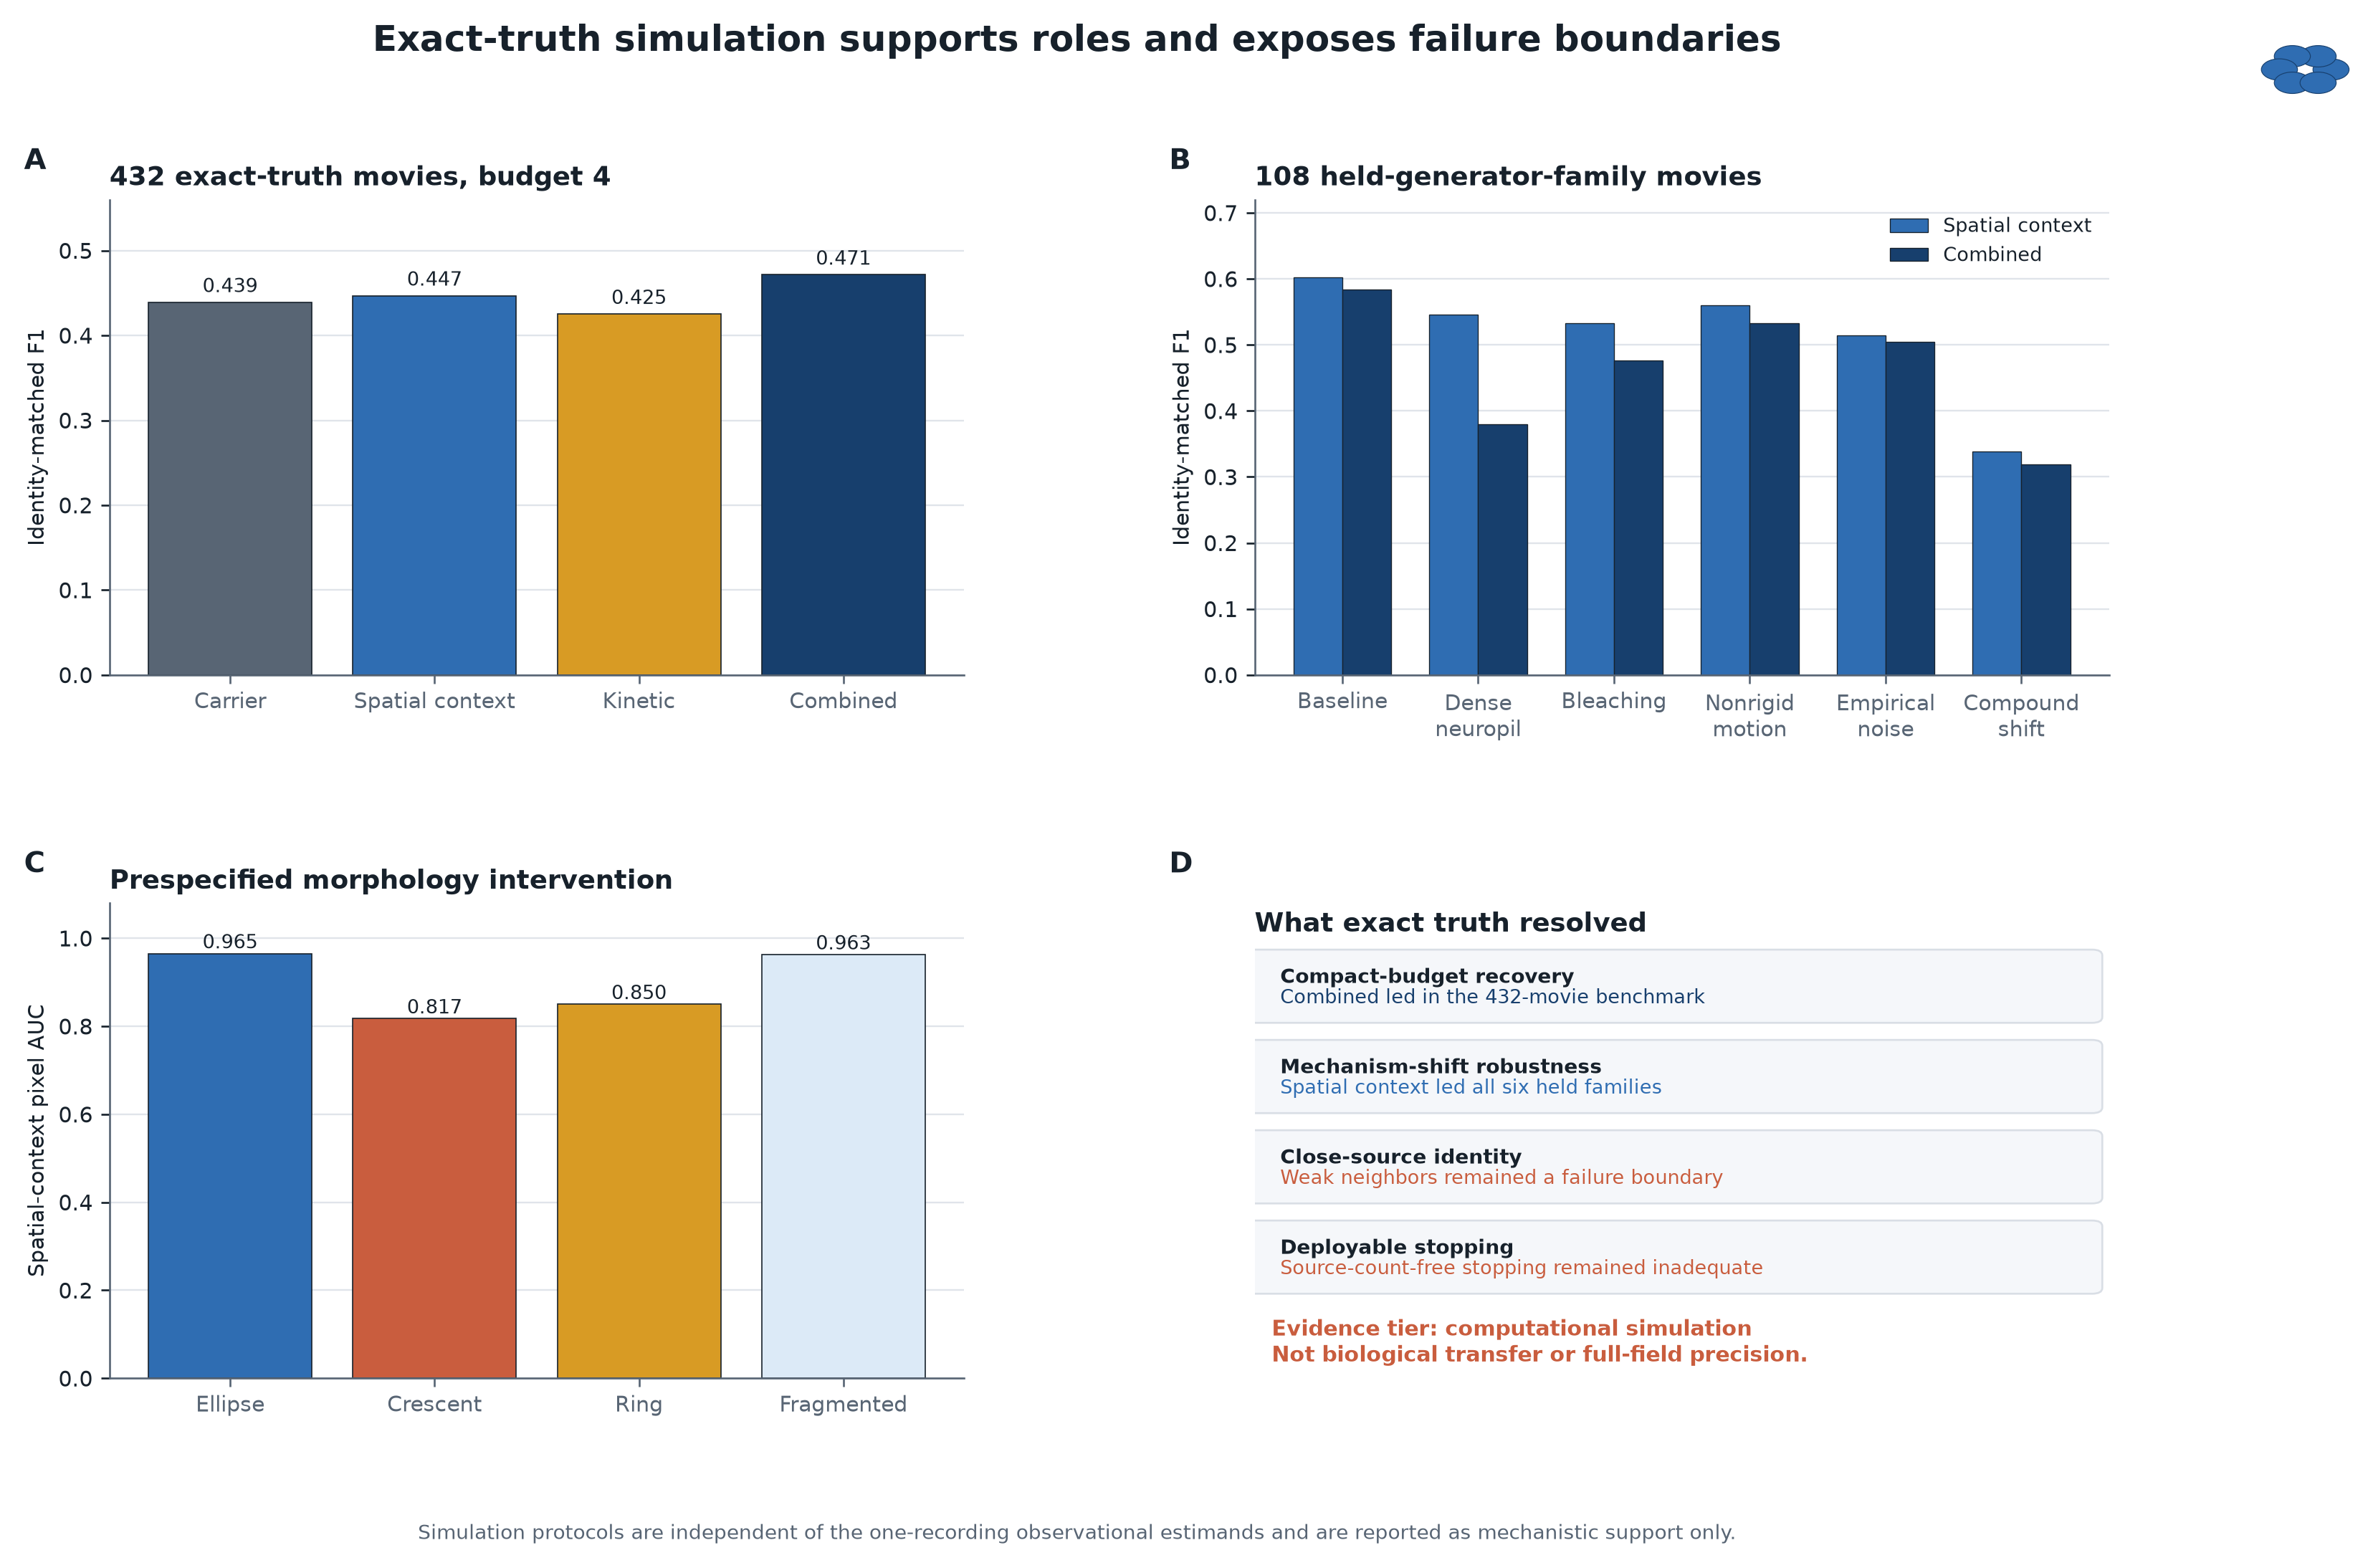
\includegraphics[width=\textwidth]{figures/venue/fig06_exact_truth_validation.png}
  \caption{Registered exact-truth simulation evidence. Panel A compares four
  frozen score stacks in \VenueMovieBenchmarkCount{} factorial movies at budget
  4. Panel B compares spatial context with equal-weight combination across six
  held generator families comprising \VenueFamilyHoldoutCount{} movies. Panel C
  shows the prespecified morphology intervention; panel D separates supported
  roles from remaining failure boundaries. Simulation is not biological
  transfer or full-field precision.}
  \label{fig:venue-exact-truth}
\end{figure*}

\subsection{The quantitative endpoints reconcile without being pooled}

Table~\ref{tab:venue-quantitative-ledger} consolidates the principal point
estimates, comparison units, and inferential boundaries. Rows are deliberately
not combined into one performance score: occurrence sensitivity, selected-site
review, numerical implementation checks, and simulated exact truth answer
different questions.

\begin{table*}[!htbp]
\centering
\caption{Quantitative result ledger. Each row retains its own population,
endpoint, and evidence boundary; values across rows are not directly
comparable performance measures.}
\label{tab:venue-quantitative-ledger}
\scriptsize
\renewcommand{\arraystretch}{0.94}
\setlength{\tabcolsep}{5.5pt}
\begin{tabularx}{\textwidth}{>{\raggedright\arraybackslash}p{0.18\textwidth}
  >{\raggedright\arraybackslash}p{0.28\textwidth}
  >{\raggedright\arraybackslash}p{0.25\textwidth}
  >{\raggedright\arraybackslash}X}
\toprule
Endpoint & Result & Unit or comparison & Boundary \\
\midrule
Known-positive sensitivity &
\VenueStrictRecovered{}/\VenueCohortOccurrences{} (\VenueStrictSensitivity)
strict; \VenueCanonicalRecovered{}/\VenueCanonicalOccurrences{}
(\VenueCanonicalSensitivity) canonical-collapsed & Any-lane union across three
per-burst B\VenuePerLaneBudget{} lists; separate grouping sensitivity & Neither
row estimates precision \\
Temporal and spatial controls & Raw AUC \VenueRawAUC{}
[\VenueRawAUCLow, \VenueRawAUCHigh]; all six compact displacement intervals
positive & Site-weighted event versus guarded quiet; matched same-field
displacement & Same-recording retrieval or localized structure \\
Candidate review & \VenueReviewDefinite{} definite,
\VenueReviewProbable{} probable, \VenueReviewUncertain{} uncertain,
\VenueReviewArtifact{} unlikely/artifact-or-noise; priority AUC
\VenueReviewPriorityAUC{} & \VenueReviewedCandidates{} detector-selected U
sites; one blinded reviewer & Provisional selected-batch yield, not precision or
validated identity count \\
Identity audit & \VenueSameIdentityCollision{} same-canonical-identity,
\VenueOtherIdentityCollision{} other-labeled-identity, and
\VenueIdentityClear{} identity-clear cases & \VenueStrictMissed{} all-lane
misses; six-pixel guard & Response gain is not recovery when identity changes \\
Frozen proposal availability & 0/\VenueIdentityClear{} identity-clear cases
available within eight pixels through per-burst B\VenueCounterfactualBudget{};
direction cosine \VenueCollisionDirectionCosine{} versus
\VenueClearDirectionCosine{}; neighbor variance explained
\VenueCollisionNeighborRtwo{} versus \VenueClearNeighborRtwo{} & Collision
versus identity-clear groups (\VenueIdentityCollision{} versus
\VenueIdentityClear{} cases) & Proposal
absence in frozen outputs; small descriptive groups \\
Numerical implementation & Long-delay maximum inversion RMS
\VenueLongDelayInversionRMSText{}; local-standardization RMSE
\VenueLSRMSEText{} and maximum error \VenueLSMaxErrorText{} &
\VenueCohortSites{} centers;
\VenueAuditFrames{} local-standardization frames & Numerical reproduction, not
source separation \\
Factorial exact truth & Combined F1 \VenueMovieCombinedFone{} versus spatial
context \VenueMovieSpatialFone{} at budget 4 & \VenueMovieBenchmarkCount{}
simulated movies; one-to-one identity matching & Computational mechanism
evidence only \\
Held-family exact truth & Mean spatial-context F1 \VenueFamilySpatialFone{}
versus combined \VenueFamilyCombinedFone{} & \VenueFamilyHoldoutCount{} movies
across six held generator families & Computational mechanism-shift evidence
only \\
Challenge morphology & Crescent spatial-context pixel AUC \VenueCrescentAUC{}
within a twelve-family challenge suite & Exact simulated truth under a
prespecified morphology intervention & Failure-boundary evidence, not
biological transfer \\
\bottomrule
\end{tabularx}
\end{table*}

\subsection{Evidence status remains distinct from run completion}

The main-paper facts are generated from \VenueFactSourceCount{} compact source
artifacts; the
source paths and hashes are recorded in a machine-readable manifest. The figure
builder independently hashes all source and output assets. Candidate review
awaits independent adjudication, cross-recording transfer is absent, and public
code/data identifiers remain unresolved. A local Feature Atlas run passed
numerical checks and is registered descriptively as NREV-EXP-0037, but its
model-annotation media audit and claim promotion remain incomplete. It is excluded from the
abstract, main Results claims, and main figures rather than being treated as a
confirmed model improvement.
